\section{Technical feasibility}\label{5_1_technicalFeasibility}
Tracking a person on a slackline is very different from a regular situation. The interplay between the range of the slackline, the movement of the line itself, unpredictable movements of the user, and his balancing actions could possibly disturb the tracking ability. This can then lead to imprecise and inaccurate tracking data. Furthermore there exists no comparable data about how to track user properly on a slackine with the Kinect.

The major point is to compare different slackline positionings and rotations regarding multiple angles and heights of the Kinect. This will then clarify how good a person can be tracked on a slackline and which is the best combination of the slackline and Kinect positioning.

\subsection{Constraints of the Kinect} 
A mentionable role plays the angle and detection range of the Kinects depth sensor regarding the length of the slackline. The sensors angle of vision is in horizontal 70 degrees and in vertical 60 degrees (Figure~\ref{fig:5_1_1_visionAngle}). Hence tracking the users height could result into problems becuause the slackline is about 30 cm off the ground, which in combination with a person on a slackline results in a higher body positioning of the person. The sensors range limits lies between 0.5 and 4.5 meters whereas the sweet spot area is between 1 up to 4 meters~\cite{MicrosoftHIG2014-mh} (Figure~\ref{fig:5_1_1_trackingRange}). Since the mobile slackline device has a length of three meters, it would fit entirely into the sweet spot tracking range. To track user for further training on a longer slackline, the depth range is not sufficient. This could be solved by using more than one Kinect device to have a larger the range. 
\begin{figure}[htb]
	\centering
	\begin{minipage}[t]{0.44\linewidth}
		\centering
		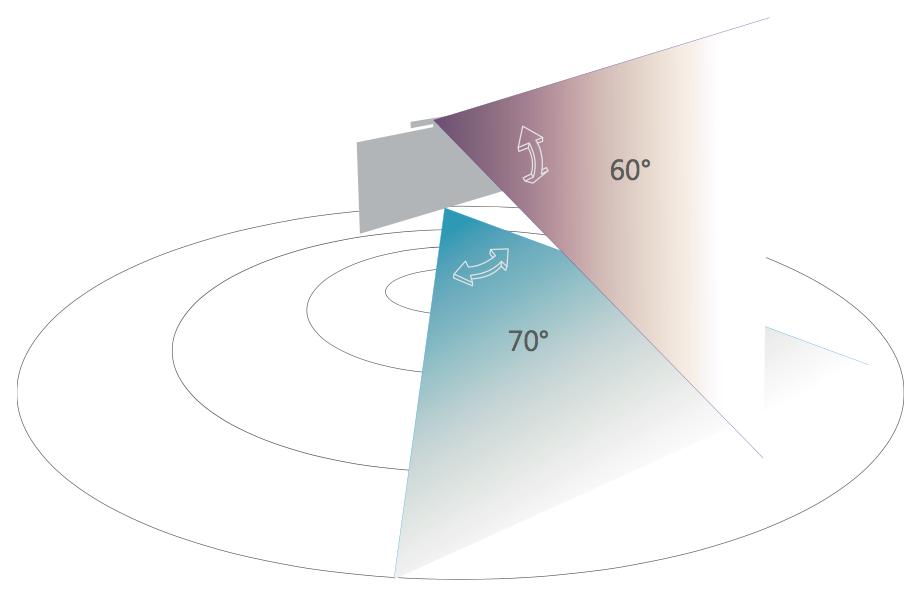
\includegraphics[width=1\linewidth]{Pictures/5_1_1_visionAngle}
		\subcaption{Angle of vision}
		\label{fig:5_1_1_visionAngle}
	\end{minipage}
	\hfill
	\begin{minipage}[t]{0.44\linewidth}
		\centering
		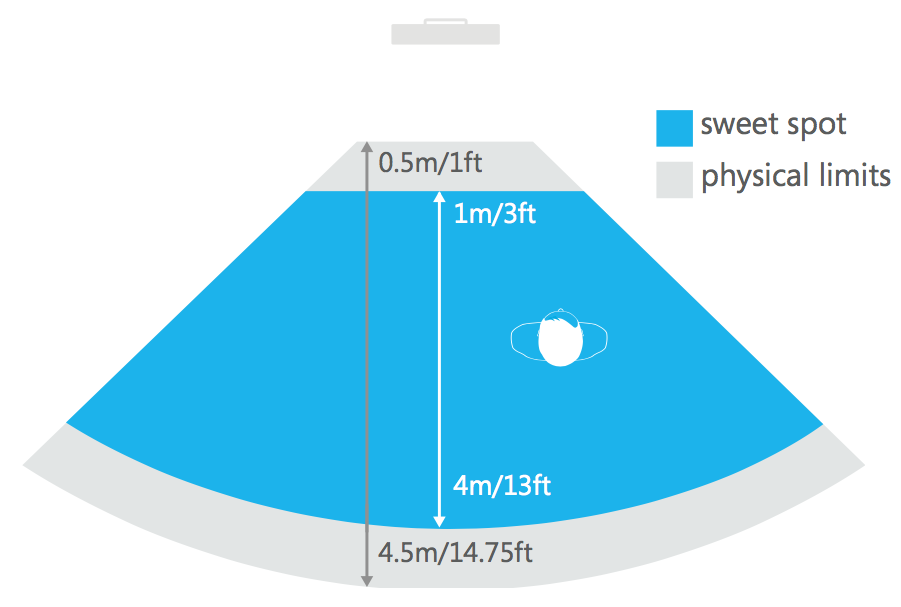
\includegraphics[width=1\linewidth]{Pictures/5_1_1_trackingRange}
		\subcaption{Kinect tracking range}
		\label{fig:5_1_1_trackingRange}
	\end{minipage}
	\caption{Sensor constraints of the Kinect v2~\cite{MicrosoftHIG2014-mh}}
	\label{fig:5_1_1_sensorConstraints}
\end{figure}

\subsection{Testing scenario}

%The test took place in the laboratory of the research group in the \textit{german reasearch center for artificial intelligence}~\footnote{\url{https://www.dfki.de/web/kontakt/dfki-saarbruecken}}. A big advantage of this is the large space to place the slackline easily in different variations. 
The slackline is placed in three positions to the Kinect: frontal (0 Degree), diagonal (45 Degree) and sideways (90 Degree) \textbf{\todo{(Figure X)}}. Each of this positions is tested regarding three different height level of the Kinect: 80 cm, 160 cm, and 240 cm. Therefore it is attached on a tripod like seen in \textbf{\todo{Figure X}}. At the end nine different combinations are covered to track a user on a slackline, which gives a good correlation of the Kinect position to the slackline. The testing person was recorded via \textit{KinectStudio}~\footnote{\url{https://developer.microsoft.com/de-de/windows/kinect/tools}}. With this one is able to record clips of a person tracked by the Kinect. Within the clips the joints of the skeletal tracking can be observed and reviewed. In the following the results discuss the feasibility and appropriate tracking positions.

\subsubsection{Slackline positioning}
\textit{\textbf{Sideways}}

The slackline positioned sideways in 90 Degrees rotated to the Kinect v2. The advantage of this is that the whole body on the slackline is in a constant line within the tracking area of the Kinect v2. With this no interference regarding the tracking distance can happen \textbf{\todo{(Figure X)}}. But the user tracking is very bad regardless of the Kinect height. This is because many body parts overlay and the Kinect v2 has problems to detect the body joints with appropriate accuracy and precision, which can be seen in \textbf{\todo{Figure X}}.

\textit{\textbf{Diagonal}}

The slackline stays diagonal in 45 Degrees to the Kinect. The frontal and end point of the slackline are now different in the vertical axis but it fits well in the tracking range \textbf{\todo{(Table X and Figure X)}}. 
%This could even result in a better trackability in matter of the depth field range, since the distance in the front shrinked and is therefore closer to the Kinect depth view. 
It shows better results in trackingability regarding the sideways positioning. Many body party does not occlude entirely but this problem is not entirely solved. It occurs that the joints of the arms and the body interfere with each other, especially at the end of the line. Also both legs occlude while stepping forwards \textbf{\todo{(Figure X)}}. This results in a bad skeletal tracking and depending on the executed exercise it can lead to detection problems.

\textit{\textbf{Frontal}}

Here the slackline is positioned frontal towards the Kinect. This resulted in the best user tracking out of the three positions. The sensor can see the full body and have nearly no problems with occlusions. Problems can occur at the starting position of the slackline since the slackline uses the entire depth range of the Kinect and the user is therefore close to the outermost range of it \textbf{\todo{(Figure X)}}.  A minor but non critical detection problem could occur with overlaying feets if the slacker stays with both on the line \textbf{\todo{(Figure X)}}.

\subsubsection{Comparing different Kinect heights}
Three main height levels were used to show the main differences of the tracking behaviour from the Kinect. It is mounted on a tripod and covers the heights of 0.80, 1.60 and 2.40 meters off the ground. 

Beginning with a height of 2.40 meters the Kinect has a very steep angle to track the slackers body on the full range of the slackline. Because of this the depth range shifts into the front like seen in \textbf{\todo{Figure X}}. Therefore if the slacker begins at the starting position on the slackline, she immediately reaches the end of the tracking area which can cause tracking problems. Also the closer she walks towards the Kinect the more occlusion happens regarding the joints.

With a height of 1.60 and 0.80 meters the entire body is fully visible in almost all ranges. The Kinect has a relatively flat angle. Because of this the slackline has to be positioned a little bit further away as former such that the body is fully visible on the entire line. This results in a more homogeneous depth range ( \textbf{\todo{Figure X}}). Problems can occur at the very end of the slackline depending on the slacker’s height. Her head or more body parts will be cropped. Therefore the slackline has to be slightly further away from the Kinect camera than on other heights. But since beginner will use the entire slackline range it can be neglected.

Overall a range between 0.80 meters up to 1.60 meters seems like the best height for the Kinect to track a person on a slacker. The tracking and view is more homogeneous and the angle flatter, which results in the possibility to use the full depth range. With a higher attachment the angle will be too steep, which results in less depth range, as well as more occlusions of body parts can occur.

\subsection{Best positioning for beginner learning purposes}
The best combination is placing the slackline frontal and having a Kinect height of 0.80 up to 1.60 meters. The Kinect can track the entire body and nearly no occlusion occur. Since only beginners are the main focus of this study, the starting position of the slackline plays an important role. Therefore for tracking purposes it is better to move the slackline closer to the camera. With this the first quarter of the slackline is cropped out of the view but the slacker can be tracked with a higher confidence at the starting position \textbf{\todo{(Figure X)}}.

\todo{\textbf{table}}